\section{Extensive Form Games}
Till now we have observed normal form games where the strategies and actions of players were simultaneous. But this form of game representation did not incorporate any notion of sequence, or time, of the action of the players. Hence, we define a different form of game called \textbf{Extensive Form Game}.\\

\begin{large}\begin{flushleft}\textbf{Extensive Form}\end{flushleft}\end{large}
\begin{itemize}
\item Players move sequentially represented as a tree
\item Include timing of moves
\item Keeps track of what each player knows when he or she makes each decision
\end{itemize}

Extensive Form is an alternative representation that makes the temporal structure explicit. It has two variants:
\begin{enumerate}
\item \textbf{Perfect-information} extensive-form games
\item \textbf{Imperfect-information} extensive-form games
\end{enumerate}

\subsection{Perfect Information Extensive Form Games}

A (finite) \textit{perfect-information game} (in extensive form) is defined by the tuple ($N, A, H, Z, \chi, \rho, \sigma, u$), where:
\begin{itemize}
\item \textbf{Players:} $N$ is a set of $n$ players
\item \textbf{Actions:} $A$ is a (single) set of actions
\item Choice nodes and label for these nodes:
	\begin{itemize}
	\item \textbf{Choice Nodes:} $H$ is a set of non-terminal choice nodes
	\item \textbf{Action Function:} $\chi : H \rightarrow 2^A$
	\item \textbf{Player Function:} $ \rho: h \rightarrow N$ assigns to each non-terminal node $h$ a player $i \in N$ who chooses an action at $h$
	\end{itemize}
\item \textbf{Terminal Nodes:} $Z$
\item \textbf{Successor Function:} $\sigma : H \times A \rightarrow H  \cup Z$ maps a choice node and an action to a new choice node or terminal node such that for all $h_1, h_2 \in H$ and $a_1,a_2 \in A$, if $\sigma(h_1,a_1) = \sigma(h_2, a_2)$ then $h_1=h_2$ and $a_1=a_2$
	\begin{itemize}
	\item Choice nodes form a tree: nodes encode history
	\end{itemize}
\item \textbf{Utility Function:} $u = (u_1, \dots , u_n); u_i: Z \rightarrow \mathbb{R}$ is a utility function for player $i$ on the terminal nodes $Z$
\end{itemize}\pagebreak
\subsubsection{Pure Strategies}
A pure strategy for a player in perfect-information game is a complete specification of which action to take at each node belonging to that player. 
\begin{flushleft}
\textbf{Definition}
\end{flushleft}
Let $G = (N, A, H, Z, \chi, \rho, \sigma, u)$ be a perfect-information extensive-form game. Then the pure strategies of player $i$ consists of the cross product $$\prod_{h\in H, \rho(h)=i} \chi(h)$$
\begin{flushleft}
\textbf{Example}
\end{flushleft}
Let's consider an example where we have a 2 dollar bill that has to be split between two players. In this, the player 1 puts forward his action from the given set \{(2,0), (1,1), (0,2)\} and the player 2 has to either accept or reject his proposal.\\
Following figure represents the corresponding tree:-
\begin{center}
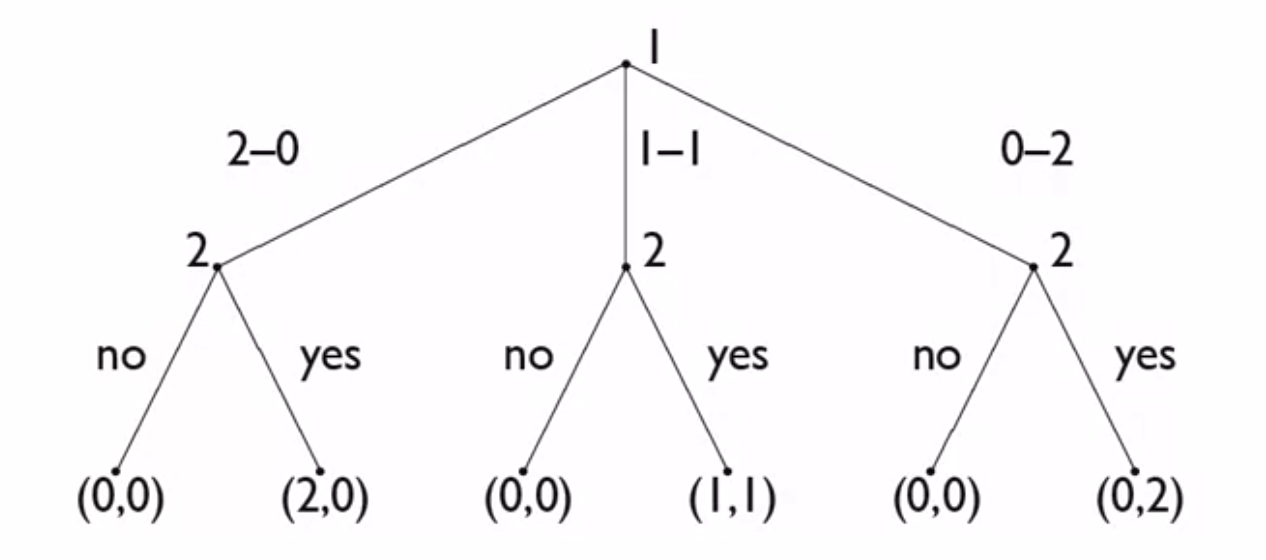
\includegraphics[scale=0.5]{sharetree}
\end{center}
Consider the pure strategies available to player 1 and 2.
\begin{itemize}
\item Player 1 can play a total of 3 pure strategies in the game
\item Player 2 has to choose between yes and no at each node. The action must belong to the set $S= \{ (a,b,c): a,b,c \in \{yes, no\}\} $. So, there are a total of $2^3 = 8$ pure strategies for the player.
\end{itemize}

The definitions of \textbf{mixed-strategy, best response} and \textbf{Nash Equilibrium} are exactly the same here.
\begin{flushleft}
\textbf{Induced Normal Form Game}
\end{flushleft}
We can transform a perfect-information game into a normal form game (as we have complete information and all the possible strategies).

In the following example, we transform a perfect-information game into normal form. The strategy profiles for corresponding players being $$S_1 =\{(A,G), (A,H), (B,G), (B,H)\} $$ $$S_2=\{ (C,E), (C,F), (D,E), (D,F)\}$$
\begin{center}
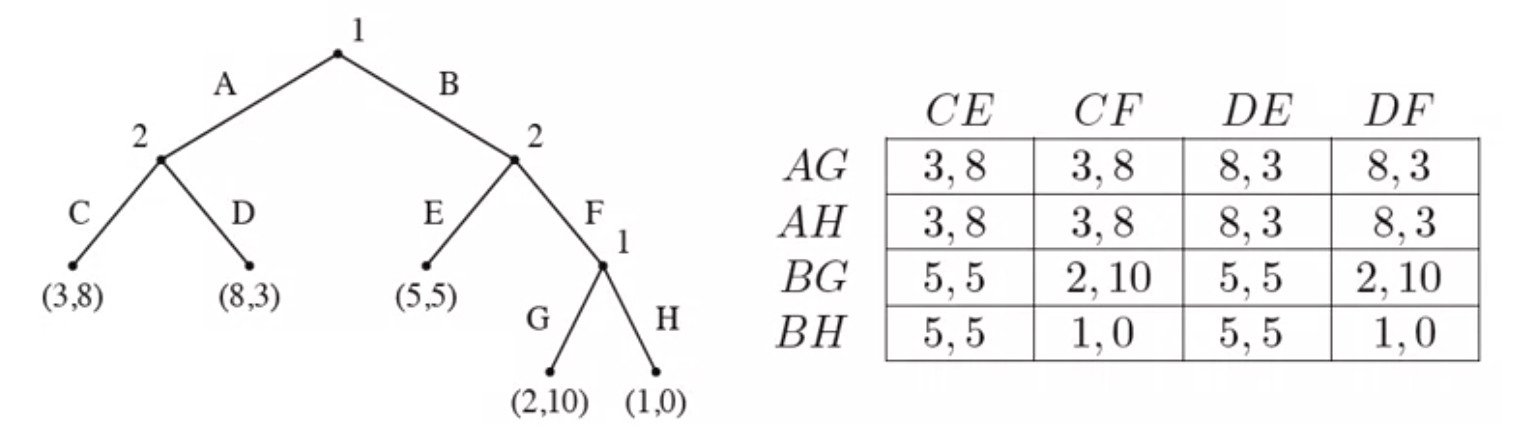
\includegraphics[scale=0.5]{normal}
\end{center}
Pure strategy Equilibria in the above example are:-\\
(A,G),(C,F)\\
(A,H),(C,F)\\
(B,H),(C,E)\\

\subsubsection{Subgame Perfection}

\textbf{Subgame}\\
The \textit{subgame of $G$ rooted at $h$} is the restriction of $G$ to the descendants of $H$.\\
\textbf{Subgames of G}\\
The \textit{set of subgames of $G$} is defined by the subgames of $G$ rooted at each of the nodes in $G$.

\begin{flushleft}
\textbf{Definition}
\end{flushleft}
$s$ is a \textit{subgame perfect equilibrium} of $G$ iff for any subgame $G'$ of $G$, the restriction of $s$ to $G'$ is a Nash Equilibrium of $G'$\\

Note:
\begin{itemize}
\item SInce $G$ is its own subgame, every \textit{subgame perfect equilibrium} is a \textit{Nash Equilibrium}
\item this definition rules out non-credible threats
\end{itemize}

\subsubsection{Backward Induction}

Backward induction in a perfect-information is an iterative process of reasoning backward in time, from the end of a problem or situation, to solve finite extensive form games, and infer a sequence of optimal actions.\\

At each stage of the game it determines the optimal strategy of the player who makes the last move in the game. Then, the optimal action of the next-to-last moving player is determined, taking the last player's action as given. This process continues backward until the best action for every point in time has been determined. Effectively, one is determining the Nash equilibrium of each subgame of the original game.

\subsection{Imperfect Information Extensive Form Games}

Unlike perfect-information games, here, an agent won't have the knowledge of the opponent's moves at every single choice node and cannot plan a best response accordingly. Rather here, players consider some choice nodes to be equivalent to each other and they won't be able to tell them apart. This can be achieved by taking all the sets of equivalent choice nodes and putting them in \textit{equivalence classes}. \\
Now, the player won't have an idea about his exact position in the tree, but knows he was at some choice node belonging to the class where he took the action with the property that each choice node in a class has the same set of actions.
\begin{flushleft}
\textbf{Definition}
\end{flushleft}
In formal terms, An \textit{imperfect-information game} (in extensive form) is a tuple $(N, A, H, Z, \chi,  \rho, \sigma, u, I)$, where
\begin{itemize}
\item $(N, A, H, Z, \chi,  \rho, \sigma, u)$ is a perfect-information extensive-form game, and
\item $I = (I_1, \dots , I_n)$, where $I_i = (I_{i,1}, \dots , I_{i, k_i})$ is an equivalence relation on $\{ h \in H, \rho(h) = i\}$ with the property that $\chi(h) = \chi(h')$ and $\rho(h) = \rho(h')$ whenever there exists a $j$ for which $h \in I_{i,j}$ and $h' \in I_{i,j}$
\end{itemize}

\subsubsection{Strategies}
\begin{flushleft}
\textbf{Pure Strategies}
\end{flushleft}
The pure strategies of player $i$ consists of the cross product $$\prod_{i, j\in I_i} \chi(I_{i,j}) $$ 
Conisder the following example game.
\begin{center}
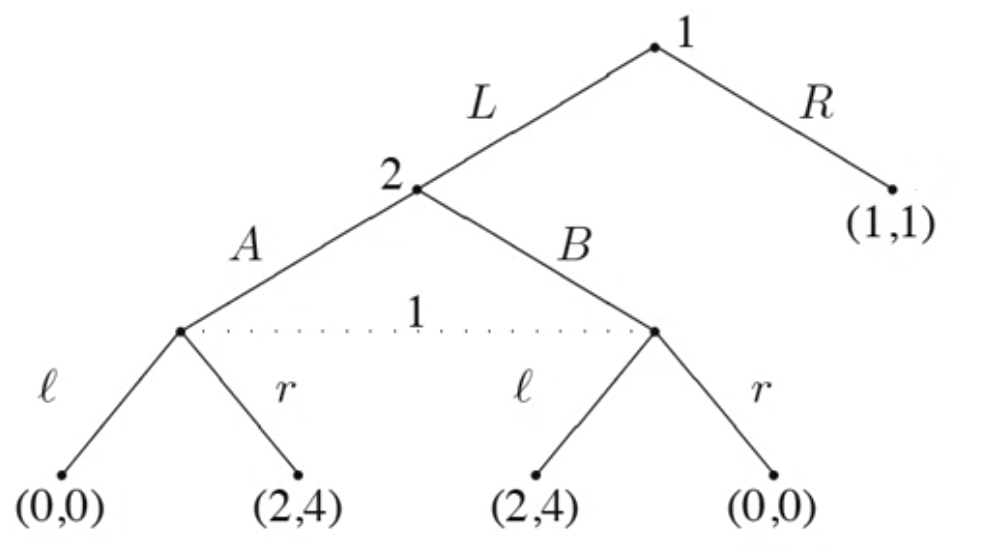
\includegraphics[scale=0.5]{imperfect}
\end{center}
\begin{itemize}
\item If Player 1 goes right, then the  game ends and the payoff is $(1,1)$
\item If Player 1 goes left, Player 2 gets to make a choice between $A$ and $B$, which is unknown to Player 1 and hence the choice nodes for Player 1 are in an equivalence class. Without knowledge of his position, Player 1 has to now move left or right.
\item Nodes of same equivalence class are marked by dotted line as above.
\item Set of pure strategies for Player 1 will be $S_1 =\{(L, l), (L, r), (R, l), (R, r)\}$ and for Player 2 will be $S_2 = \{A, B\}$
\end{itemize}

\subsubsection{Normal-Form Games}
We can represent normal form games in the tree format of imperfect-information game. Consider the \textbf{Prisoners' Dilemma Game} in section 4.3. The game can be represented as a tree in the following manner-
 \begin{center}
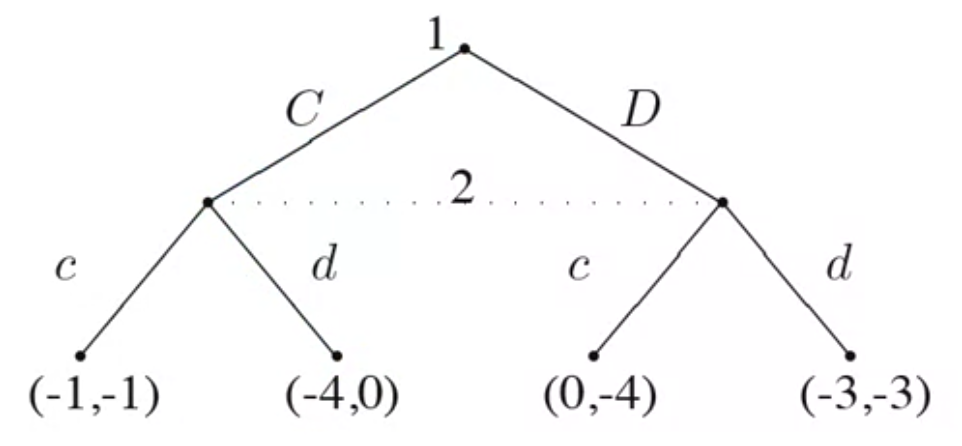
\includegraphics[scale=0.5]{norm}
\end{center}
\begin{itemize}
\item Notice that the order doesn't matter as to who is at the root node because time isn't playing a role in this game
\item The other player has no idea about the first player's moves, hence he has an equivalence class to choose from.
\end{itemize} 
\subsubsection{Mixed and Behavioural Strategies}
There are two meaningfully different kinds of randomized strategies in imperfect-information extensive form games-
\begin{itemize}
\item \textbf{Mixed strategies}-  assign a probability distribution over pure strategies
\item \textbf{Behavioural strategies}- assign, independently for each information set, a probability distribution over actions
\end{itemize}